%!TeX root=20_Hauptteil.tex

\chapter{Theoretische Grundlagen}

ZZum besseren Verständnis der vorliegenden Arbeit werden im folgenden Kapitel die theoretischen Grundlagen erläutert.
Es werden grundlegende Begriffe aus den Bereichen der Robotik, der Sensorik sowie der visuellen Navigation eingeführt.
Darüber hinaus wird gesondert auf den verwendeten Flugcontroller, die zugrundeliegenden Koordinatensysteme sowie die relevanten Transformationen eingegangen. 


\section{Grundlagen Unbemannter Flugroboter am Beispiel der Holybro X650}
Unter einem unbemannten Luftfahrzeug \gls{uav}, umgangssprachlich auch als Drohne bezeichnet, versteht man ein Fluggerät, welches ohne einen menschlichen Piloten an Bord betrieben werden kann.
Dabei können \gls{uav}s entweder ferngesteuert von einem menschlichen Operator oder vollständig autonom durch einen bordeigenen Computer geführt werden.
Die Anfänge unbemannter Luftfahrzeuge reichen bis in die 1910er Jahre zurück, wo sie vorrangig für militärische Zwecke eingesetzt wurden.
Ab den 2000er Jahren fanden \gls{uav}s zunehmend Eingang in zivile Anwendungsgebiete, wie beispielsweise die Katastrophenhilfe. \cite[S. 1--3]{Studiawan2026}

\subsection{Aufbau der Holybro X650}
\textbf{Grundrahmen} Der Grundrahmen eines UAV dient als mechanische Basis für die Montage aller weiteren Komponenten.
Das Design des Rahmens beeinflusst maßgeblich die Flugeigenschaften des Geräts.
Das in dieser Arbeit verwendete Modell ist als Senkrechtstarter konzipiert und basiert auf einem X-förmigen Quadcopter-Rahmen.
Die wesentlichen Bestandteile des Rahmens umfassen die Ausleger, das Landegestell sowie die zentrale Montageplattform für die Elektronik.
Die Holybro X650 weist eine Diagonale von 650 mm auf.
Abbildung \ref{fig:roll_pitch_yaw} zeigt ein Bild der Holybro X650.
 \cite{Wu2021} \cite{holybro_x650}

\noindent
\textbf{Antriebssystem} Das Antriebssystem besteht aus vier Elektromotoren, die jeweils an einem der Ausleger montiert sind.
An den Motoren sind Propeller befestigt, welche den erforderlichen Auftrieb erzeugen.

\noindent
\textbf{Flugcontroller} Der Flugcontroller bildet das zentrale Steuerungselement eines UAV.
Er setzt eingehende Steuerbefehle in konkrete Ansteuersignale um, die an die Motoren weitergeleitet werden.
In Kapitel \ref{sec:PX4 Autopilot} wird näher auf den verwendeten Flugcontroller eingegangen.

\noindent
\textbf{Energieversorgung} Die Energieversorgung erfolgt über einen \gls{lipo} mit einer Nennspannung von 14,8 V.
Das verbaute Power Module wandelt diese Spannung auf 5,2 V, mit welcher sowohl die Steuerelektronik als auch die Motoren versorgt werden.

\noindent
\textbf{Nutzlast} Das maximale Abfluggewicht der Holybro X650 beträgt 6,3 kg, wobei der flugfertige Grundrahmen bereits ein Eigengewicht von 4,3 kg aufweist.
Daraus ergibt sich eine maximale Nutzlast von 2 kg (ohne Akku). \cite{holybro_x650}

\section{Koordinatensysteme und Transformationen}
Dieses Kapitel behandelt die verschiedenen Koordinatensysteme, die in dieser Arbeit relevant sind.
Dabei wird zwischen dem Welt-, Roboter-, Kamera- und Fiducialkoordinatensystem unterschieden.
Weiterhin werden die grundlegenden Konzepte zur Repräsentation von Position und Orientierung im Raum erläutert.
Abschließend wird auf die notwendigen Koordinatentransformationen eingegangen.

\subsection{Vergleich von Welt-, Roboter-, Kamera- und Fiducialkoordinatensystem}
Ein Koordinatensystem ist ein mathematisches Konstrukt, das zur eindeutigen Beschreibung der Lage von Punkten im Raum verwendet wird.
Zur Beschreibung von Bewegungen ist die Festlegung eines Koordinatensystems von entscheidender Bedeutung.
Es besteht aus einem Bezugspunkt, dem Ursprung, sowie drei orthogonalen Achsen, die als X-, Y- und Z-Achse bezeichnet werden.
In dieser Arbeit wird standardmäßig das rechtshändige Koordinatensystem verwendet. \cite[S. 17]{ISO8855}
Mathematisch wird der Zusammenhang durch
\begin{equation}
\mathbf{Z} = \mathbf{X} \times \mathbf{Y}
\label{eq:rechte_hand_regel}
\end{equation}
dargestellt.
In dieser Arbeit werden die Achsen entsprechend des informellen Industriestandards wie folgt dargestellt: X-Achse in Rot, Y-Achse in Grün und Z-Achse in Blau.
Ein Überblick über die in dieser Arbeit verwendeten Koordinatensysteme ist in Abbildung \ref{fig:Koordinatensysteme} dargestellt.

\begin{figure}[htbp]
\centering
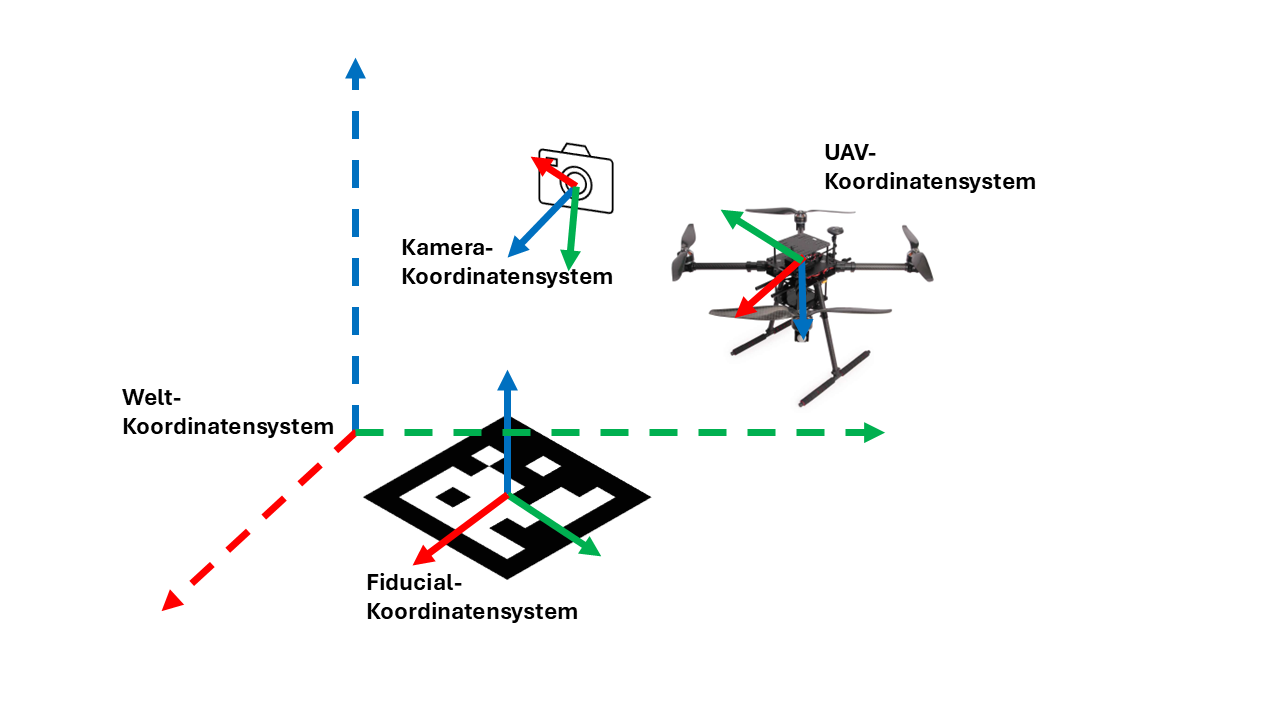
\includegraphics[width=1.0\textwidth]{Bilder/Koordinatensysteme.png}
\caption{Vergleich der Koordinatensysteme \cite{holybro_x650}}
\label{fig:Koordinatensysteme}
\end{figure}
\FloatBarrier

Das Weltkoordinatensystem dient als globaler Referenzrahmen, in dem die Position aller Objekte beschrieben wird.
Der Ursprung dieses Koordinatensystems kann frei gewählt werden und wird durch die Variable $O_0$ repräsentiert.
Die Achsen werden durch $X_0$, $Y_0$ und $Z_0$ dargestellt \cite[S. 4]{ISO9787}.

Das UAV-Koordinatensystem ist in der Regel vom Hersteller vorgegeben und richtet sich in diesem konkreten Fall nach dem Flugregler.
In der zugehörigen Dokumentation wird angegeben, dass die X-Achse ($X_u$) nach vorne, die Y-Achse ($Y_u$) 
nach rechts und die Z-Achse ($Z_u$) nach unten zeigt.
Der Ursprung dieses Koordinatensystems ($O_u$) befindet sich im Zentrum des Flugreglers \cite{PX4Frames}.

Das Kamerakoordinatensystem ist in der Regel so definiert, dass die Z-Achse ($Z_c$) entlang der optischen Achse der Kamera zeigt, 
die X-Achse ($X_c$) nach rechts auf der Bildebene und die Y-Achse ($Y_c$) nach unten auf der Bildebene zeigt.
Der Ursprung ($O_c$) befindet sich im optischen Zentrum der Kamera. \cite[S. 44]{Szeliski2022}

Das Fiducialkoordinatensystem ist in dieser Arbeit so definiert, dass sich der Ursprung ($O_f$) im Mittelpunkt der Fiducialmarke befindet.
Die Z-Achse ($Z_f$) zeigt senkrecht aus der Markerebene heraus, die X-Achse ($X_f$) zeigt nach rechts in der Markerebene und die Y-Achse ($Y_f$) 
zeigt nach oben in der Markerebene.



\subsection{Repräsentation von Position und Orientierung}
In diesem unterkapitel wird das verwendetet \gls{uav} als starrer Körper betrachtet. 
Die vollständige Beschreibung der Lage eines starren Körpers im Raum erfolgt durch seine Position und Orientierung \cite[38]{Siciliano2009}.

Die Position eines Körpers wird durch den Vektor
\begin{equation}
\mathbf{p} = (x, y, z)^T
\label{eq:position_vektor}
\end{equation}
beschrieben. 
Wobei die Koordinaten einen bestimmten Koordinatensystem zugeordnet sind. 

Die Orientierung eines Körpers kann auf verschiedene Weisen dargestellt werden. 
Im Folgenden werden die zum Verständnis dieser Arbeit relevanten Darstellungsformen erläutert.
Grundsätzlich kann sich ein Körper um drei Achsen drehen, was durch die Euler-Winkel Roll ($\phi$), Pitch ($\theta$) und Yaw ($\psi$) beschrieben wird.
Abbildung \ref{fig:roll_pitch_yaw} zeigt die Definition dieser Winkel am Beispiel der Holybro X650.
Die Pfeilrichtung entspricht der positiven Drehrichtung im rechtshändigen Koordinatensystem.
\begin{figure}[htbp]
   \centering
   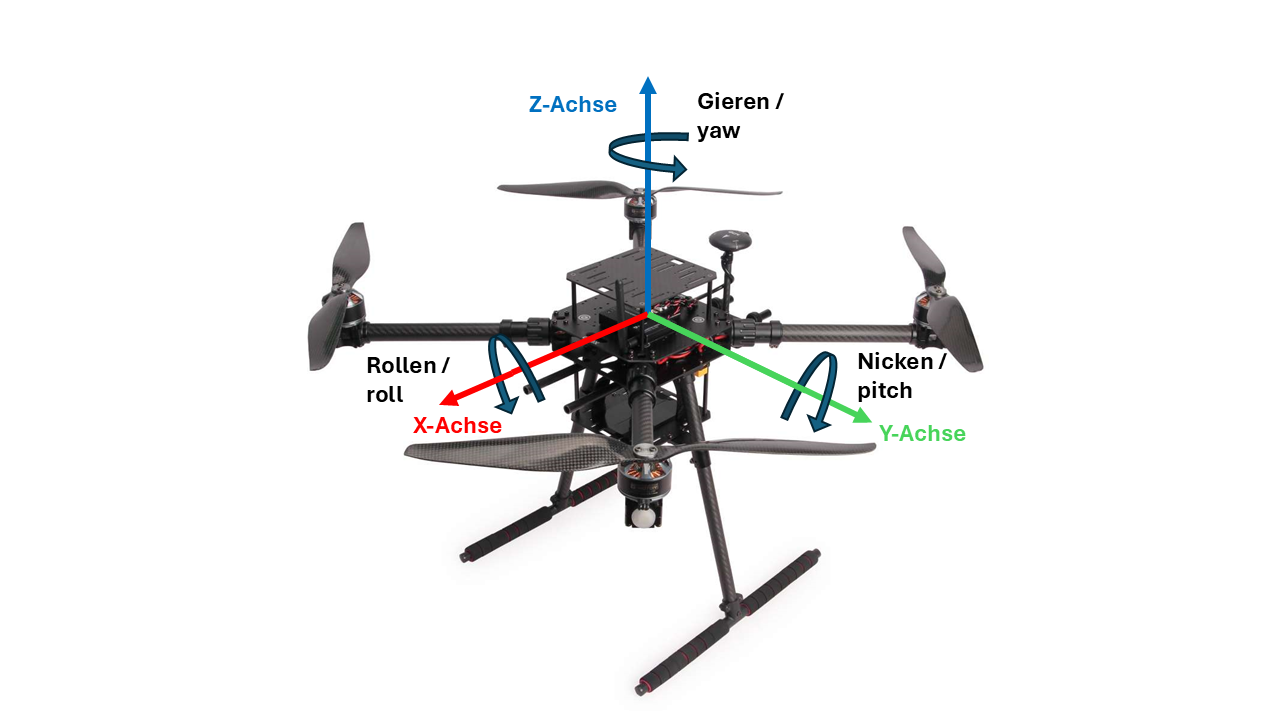
\includegraphics[width=1.0\textwidth]{Bilder/Roll_Yaw_Pitch.png}
   \caption{Roll, Pitch und Yaw am Beispiel Holybro X650 \cite{holybro_x650}}
   \label{fig:roll_pitch_yaw}
\end{figure}
\FloatBarrier

Die folgenden Ausführungen zu Quaternionen beziehen sich auf \cite[15-16]{2016}.
Weiterhin kann die Orientierung als sogenanntes Quaternion dargestellt werden.
Quaternionen bieten gegenüber Euler-Winkeln den Vorteil, dass sie keine Singularitäten (Gimbal Lock) aufweisen.
Quaternionen stellen eine Erweiterung des komplexen Zahlenraums dar und werden durch Gleichung \ref{eq:quaternion} definiert.
\begin{equation}
\mathbf{q} = w + ix + jy + kz
\label{eq:quaternion}
\end{equation}
wobei die Komponenten $w$, $x$, $y$ und $z$ reelle Zahlen sind Skalare sind und $i$, $j$ und $k$ die imaginären Einheiten darstellen.
Die Imaginären Einheiten erfüllen die folgenden Multiplikationsregeln:
\begin{equation}
ii = jj = kk = ijk = -1
\label{eq:quaternion_regeln}
\end{equation}

\begin{equation}
ij = k , \quad jk = i , \quad ki = j
\label{eq:quaternion_regeln2}
\end{equation}

\begin{equation}
ji = -k , \quad kj = -i , \quad ik = -j
\label{eq:quaternion_regeln3}
\end{equation}

Addition und Multiplikation von Quaternionen werden entsprechend den Formeln \ref{eq:quaternion_addition} und \ref{eq:quaternion_multiplikation} definiert.
\begin{equation}
q_1 + q_2 = (w_1 + w_2) + i(x_1 + x_2) + j(y_1 + y_2) + k(z_1 + z_2)
\label{eq:quaternion_addition}
\end{equation}
\begin{equation}
\begin{split}
q_1 \cdot q_2 = &(w_1 w_2 - x_1 x_2 - y_1 y_2 - z_1 z_2) \\
+ &i(w_1 x_2 + x_1 w_2 + y_1 z_2 - z_1 y_2) \\
+ &j(w_1 y_2 - x_1 z_2 + y_1 w_2 + z_1 x_2) \\
+ &k(w_1 z_2 + x_1 y_2 - y_1 x_2 + z_1 w_2)
\end{split}
\label{eq:quaternion_multiplikation}
\end{equation}

Das Einheitsquaternion oder auch Rotationsquaternion $\mathbf{q}$ beschreibt eine Rotation um den Winkel $\phi$ 
um eine normierte Rotationsachse $\mathbf{v} = (v_x, v_y, v_z)^T$ und wird durch Gleichung \ref{eq:einheitsquaternion} beschrieben. 

\begin{equation}
\mathbf{q} = \left(\cos\frac{\phi}{2},\ \mathbf{v} \cdot \sin\frac{\phi}{2}\right) = \left(\cos\frac{\phi}{2},\ v_x \sin\frac{\phi}{2},\ v_y \sin\frac{\phi}{2},\ v_z \sin\frac{\phi}{2}\right)
\label{eq:einheitsquaternion}
\end{equation}

Die Konjunktion eines Quaternions ist analog zu den komplexen Zahlen mit der Gleichung \ref{eq:quaternion_konjungiert} beschrieben. 
\begin{equation}
\bar{\mathbf{q}} = (w, -x, -y, -z)
\label{eq:quaternion_konjugiert}
\end{equation}

Für die Rotation eines beliebigen Punktes $\mathbf{p} = (0, p_x, p_y, p_z)$ um ein 
Rotationsquaternion $\mathbf{q}$ kann nun die Gleichung \ref{eq:quaternion_rotation} angewendet werden. \cite[S. 112]{Quan2017}

\begin{equation}
\mathbf{p}' = \mathbf{q} \cdot \mathbf{p} \cdot \bar{\mathbf{q}}
\label{eq:quaternion_rotation}
\end{equation}

\subsection{Transformation von Koordinatensystemen}

\subsection{Repräsentation von Position}
Ein Punkt in einem Raum wird durch einen Vektor 

\subsection{Repräsentation von Orientierung}

 

\section{Autopilot PX4-6C}
\label{sec:PX4 Autopilot}
Hier einfach schreiben...
\subsection{Architektur}
Hier einfach schreiben...

\subsection{Sensorintegration}
Hier einfach schreiben...

\subsection{Kommunikationsschnittstellen}
Hier einfach schreiben...

\subsection{Echtzeitfähikgkeit}


\subsection{Vergleich von Kamera-, Roboter- und Weltkoordinatensystem}

\subsection{Transformation von Koordinatensystemen}

\section{Visuelle Navigation}

\subsubsection{Sensorik zur visuellen Navigation}

\subsubsection{Grundlagen der Fiduccial-Erkennung}
\subsubsection{PNP-Fehler}

\subsubsection{Visuelle Odometrie}




